% Drawing 138/06-45 -- folder 138, batch 06, archive page 118 (PDF page 119).
% Transcription: une étoile à six branches, $\underline{\underline{\mathbb{D}_6}}$ ; séparée par une double barre, une étoile à quatre branches avec une boucle, $\mathbb{Z}_2$ ; un tripode avec une boucle, $\mathbb{Z}_2$ ; une boucle traversée à trois arêtes pendantes, $\mathbb{Z}_2 \times \mathbb{Z}_2$ ; deux boucles accolées à deux arêtes, $\mathbb{Z}_2$ ; une boucle contenant un point, avec deux arêtes intérieures, $\mathbb{Z}_2$ ; deux boucles accolées traversées d'un segment, $\mathbb{Z}_2 \times \mathbb{Z}_2$ ; deux boucles et une arête, $1$ ; trois boucles, $\mathfrak{S}_3$ ; une boucle dans une boucle, $\mathbb{Z}_2$ ; au crayon, dans un enclos, deux boucles traversées d'un segment, $\mathbb{Z}_2 \times \mathbb{Z}_2$, avec le type (d'une autre encre) $\bigl(6, \begin{smallmatrix}2_2\\1_2\end{smallmatrix}, \begin{smallmatrix}4\\1_2\end{smallmatrix}\bigr)$.
% Kind: table of small maps with automorphism groups (degree 6, a). Method 2 (schematic redraw from the facsimile). Status: partial.
% Notes: Degree 6, a): a star with six branches, D_6 (double underlined), then after a double bar: a star with four branches and a loop, Z_2; a tripod with a loop, Z_2; a loop crossed with three hanging edges, Z_2 x Z_2; two joined loops with two edges, Z_2; a loop containing a point, with two inner edges, Z_2; two joined loops crossed by a segment, Z_2 x Z_2; two loops and an edge, 1 (circled); three loops, S_3 (circled); a loop in a loop, Z_2; in pencil, inside an enclosure, two loops crossed by a segment, Z_2 x Z_2, with the type (6, 2_2 1_2, 4 1_2) in another ink. The scribble at the right edge is left out. The shapes of the multi-loop maps are a reading. Each small map carries its automorphism group as written (given as labels, since the transcription names them); vertex positions and loop shapes approximate.
% Coordinates: 1 unit = 1 mm = 1/100 of the crop width (bbox in page fractions: [0.156, 0.072, 0.895, 0.286]).
% Redrawn by Claude (claude-opus-5-5), issue #73, 2026-11-07; not checked by a human; not compiled (no TeX in the session).
% Rights: reproduces part of the work -- behind RENDER_TRANSCRIPTS, never published by itself.
\documentclass[tikz,border=3pt]{standalone}
\usepackage{amsmath,amssymb}
\usetikzlibrary{patterns,arrows.meta}
\tikzset{pencil/.style={black!45}, struck/.style={black!35}, mark/.style={circle,draw,inner sep=1.3pt}, pt/.style={circle,fill,inner sep=0.9pt}, opt/.style={circle,draw,fill=white,inner sep=1.1pt}}
\begin{document}
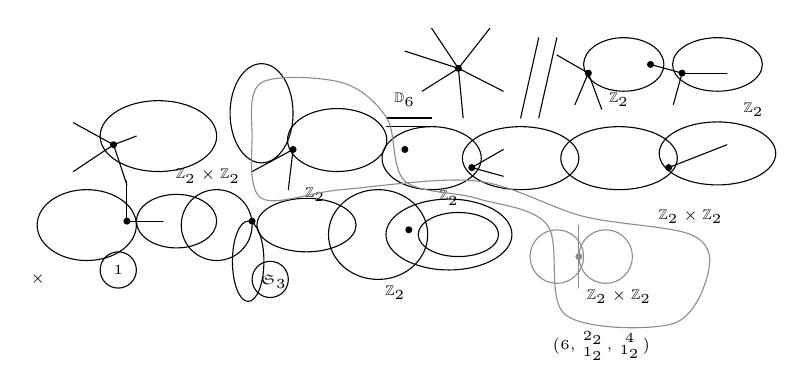
\begin{tikzpicture}[x=1mm,y=1mm,line cap=round,line join=round,font=\scriptsize]
\draw (55.7,-6.2) -- (52.3,-1.1);
\draw (55.7,-6.2) -- (59.7,-1.1);
\draw (55.7,-6.2) -- (61.4,-9.1);
\draw (55.7,-6.2) -- (56.3,-12.5);
\draw (55.7,-6.2) -- (51.1,-9.1);
\draw (55.7,-6.2) -- (48.9,-4);
\node[pt] at (55.7,-6.2) {};
\node[inner sep=1pt] at (48.9,-10.2) {\tiny $\mathbb{D}_6$};
\draw (46.6,-12.5) -- (52.3,-12.5);
\draw (46.6,-13.6) -- (52.3,-13.6);
\draw (65.9,-2.3) -- (63.6,-12.5);
\draw (68.2,-2.3) -- (65.9,-12.5);
\draw (76.7,-5.7) ellipse[x radius=5.1, y radius=3.4];
\draw (72.2,-6.8) -- (68.2,-4.5);
\draw (72.2,-6.8) -- (70.5,-10.8);
\draw (72.2,-6.8) -- (73.9,-11.4);
\node[pt] at (72.2,-6.8) {};
\node[inner sep=1pt] at (76.1,-10.2) {\tiny $\mathbb{Z}_2$};
\draw (88.6,-5.7) ellipse[x radius=5.7, y radius=3.4];
\draw (84.1,-6.8) -- (80.1,-5.7);
\draw (84.1,-6.8) -- (83,-10.8);
\draw (84.1,-6.8) -- (89.8,-6.8);
\node[pt] at (84.1,-6.8) {};
\node[pt] at (80.1,-5.7) {};
\node[inner sep=1pt] at (93.2,-11.4) {\tiny $\mathbb{Z}_2$};
\draw (17.6,-14.8) ellipse[x radius=7.4, y radius=4.5];
\draw (11.9,-15.9) -- (6.8,-13.1);
\draw (11.9,-15.9) -- (6.8,-19.3);
\draw (11.9,-15.9) -- (13.6,-21);
\draw (11.9,-15.9) -- (14.8,-14.8);
\node[pt] at (11.9,-15.9) {};
\node[inner sep=1pt] at (23.9,-19.9) {\tiny $\mathbb{Z}_2\times\mathbb{Z}_2$};
\draw (30.7,-11.9) ellipse[x radius=4, y radius=6.3];
\draw (40.3,-15.3) ellipse[x radius=6.3, y radius=4];
\draw (34.7,-16.5) -- (34.1,-21.6);
\draw (34.7,-16.5) -- (29.5,-19.3);
\node[pt] at (34.7,-16.5) {};
\node[inner sep=1pt] at (37.5,-22.2) {\tiny $\mathbb{Z}_2$};
\draw (52.3,-17.6) ellipse[x radius=6.3, y radius=4];
\draw (63.6,-17.6) ellipse[x radius=7.4, y radius=4];
\draw (57.4,-18.8) -- (61.4,-19.9);
\draw (57.4,-18.8) -- (61.4,-16.5);
\node[pt] at (57.4,-18.8) {};
\node[pt] at (48.9,-16.5) {};
\node[inner sep=1pt] at (54.5,-22.7) {\tiny $\mathbb{Z}_2$};
\draw (76.1,-17.6) ellipse[x radius=7.4, y radius=4];
\draw (88.6,-17) ellipse[x radius=7.4, y radius=4];
\draw (82.4,-18.8) -- (89.8,-15.9);
\node[pt] at (82.4,-18.8) {};
\node[inner sep=1pt] at (85.2,-25) {\tiny $\mathbb{Z}_2\times\mathbb{Z}_2$};
\draw (8.5,-26.1) ellipse[x radius=6.3, y radius=4.5];
\draw (19.9,-25.6) ellipse[x radius=5.1, y radius=3.4];
\draw (13.6,-20.5) -- (13.6,-25.6);
\draw (13.6,-25.6) -- (18.2,-25.6);
\node[pt] at (13.6,-25.6) {};
\draw (12.5,-31.8) circle[radius=2.3];
\node[inner sep=1pt] at (12.5,-31.8) {\tiny $1$};
\node[inner sep=1pt] at (2.3,-33) {\tiny $\times$};
\draw (25,-26.1) ellipse[x radius=4.5, y radius=4.5];
\draw (36.4,-26.1) ellipse[x radius=6.3, y radius=3.4];
\draw (29,-30.7) ellipse[x radius=2, y radius=5.1];
\node[pt] at (29.5,-25.6) {};
\draw (31.8,-33) circle[radius=2.3];
\node[inner sep=1pt] at (32.2,-33.3) {\tiny $\mathfrak{S}_3$};
\draw (45.5,-27.3) ellipse[x radius=6.3, y radius=5.7];
\draw (54.5,-27.3) ellipse[x radius=8, y radius=4.5];
\draw (55.7,-27.3) ellipse[x radius=5.1, y radius=2.8];
\node[pt] at (49.4,-26.7) {};
\node[inner sep=1pt] at (47.7,-34.7) {\tiny $\mathbb{Z}_2$};
\draw[pencil] plot[smooth cycle, tension=0.55] coordinates {(30.7,-8) (40.9,-8) (46.6,-12.5) (48.9,-20.5) (58,-22.7) (67,-26.1) (69.3,-37.5) (83,-38.6) (87.5,-31.8) (85.2,-27.3) (71.6,-25) (58,-20.5) (40.9,-21.6) (30.7,-22.7) (29.5,-14.8)};
\draw[pencil] (68.2,-30.1) circle[radius=3.4];
\draw[pencil] (74.4,-30.1) circle[radius=3.4];
\draw[pencil] (71,-26.1) -- (71,-34.1);
\node[pt,pencil] at (71,-30.1) {};
\node[inner sep=1pt] at (76.1,-35.2) {\tiny $\mathbb{Z}_2\times\mathbb{Z}_2$};
\node[inner sep=1pt] at (73.9,-41.5) {\tiny $\bigl(6,\begin{smallmatrix}2_2\\1_2\end{smallmatrix},\begin{smallmatrix}4\\1_2\end{smallmatrix}\bigr)$};
\end{tikzpicture}
\end{document}
